\begin{Ueberlieferung}% 
{\textit{L}}Konzept: LH XXXVII 3 Bl. 77-78. 1 Bog. 2\textsuperscript{o}. 2 S. auf Bl. 78, Textfolge: Bl. 78~v\textsuperscript{o}, 78~r\textsuperscript{o}.
Bl. 77~r\textsuperscript{o} überliefert N.~45\textsubscript{3}.
% De vectibus conjugatis
Bl. 77~v\textsuperscript{o} ist leer. 
Je ein verschiedenes Wasserzeichen auf Bl.~77 und 78.\\%
Cc 2, Nr. 1213 D
\end{Ueberlieferung}
%
\vspace*{8mm}
% \begin{Datierungsgruende}%
% ?? Wasserzeichen auf 77 und 78
% \end{Datierungsgruende}
%
%\pstart
%[78~v\textsuperscript{o}]
%\pend
\count\Afootins=1200
\count\Bfootins=1200
\count\Cfootins=1200
\pstart%
\noindent%
[78~v\textsuperscript{o}]
\edtext{In vectem\protect\index{Sachverzeichnis}{vectis} $AD$}{\lemma{}\Bfootnote{%
Duae sunto bila \textit{streicht Hrsg.}\ \textbar \ In\ \textit{(1)}\ brachium\protect\index{Sachverzeichnis}{brachium} $AC$\  \textit{(2)}\ vectem\protect\index{Sachverzeichnis}{vectis} $AD$\ \textit{L}}}
%
impingit alius vectis\protect\index{Sachverzeichnis}{vectis} $CB$ quo sublato et 
\edtext{alter $AD$ sustollitur.}{\lemma{alter $AD$}\Bfootnote{\textit{(1)}\ tollitur \textit{(2)}\ sustollitur. \textit{L}}}
Dantur 2 rectae $AC$ et $CB$ aequales. Datur et recta $CF$ et $AF=FB$. Datur ergo et angulus \textit{CBF}, vel \textit{CAF}. Attollatur $BC$ in $BD$ per altitudinem $DE$, infinite parvam. Pondus\protect\index{Sachverzeichnis}{pondus} quod in $C$ esse fixum intelligebatur translatum erit in $G$ per altitudinem $GH$ etiam infinite parvam. Quaeritur ratio $DE$ ad $GH$ lineis veris expressa.
\pend
\pstart
Producatur $DC$ dum occurrat ipsi $AB$ in $L$ patet rectam $BC$ esse ipsi $BC$
\edtext{vel $BD$}{\lemma{}\Bfootnote{vel $BD$  \textit{erg.} \textit{L}}} 
perpendicularem, quia $BC$ et $BM,$ cui perpendicularis est coincidant, sive quod idem est differentiam habent assignatam quavis minorem. Eadem $GC$ producta in $N$ est perpendicularis ipsi $AC$ vel $AD$.
\pend
\pstart
Caeterum ut inveniamus $GH$ procedamus velut si linea $DE$ esset vera, dataeque $AF=FB,$ et $CF.$ Ante omnia \rule[-4mm]{0mm}{10mm}$\displaystyle\frac{DE}{CE}=\frac{CF}{FL}$
ergo posita $DE=1,$ erit
$\displaystyle CE=\frac{FL}{CF}.$
\pend
\vspace{1em}
\pstart
\centering
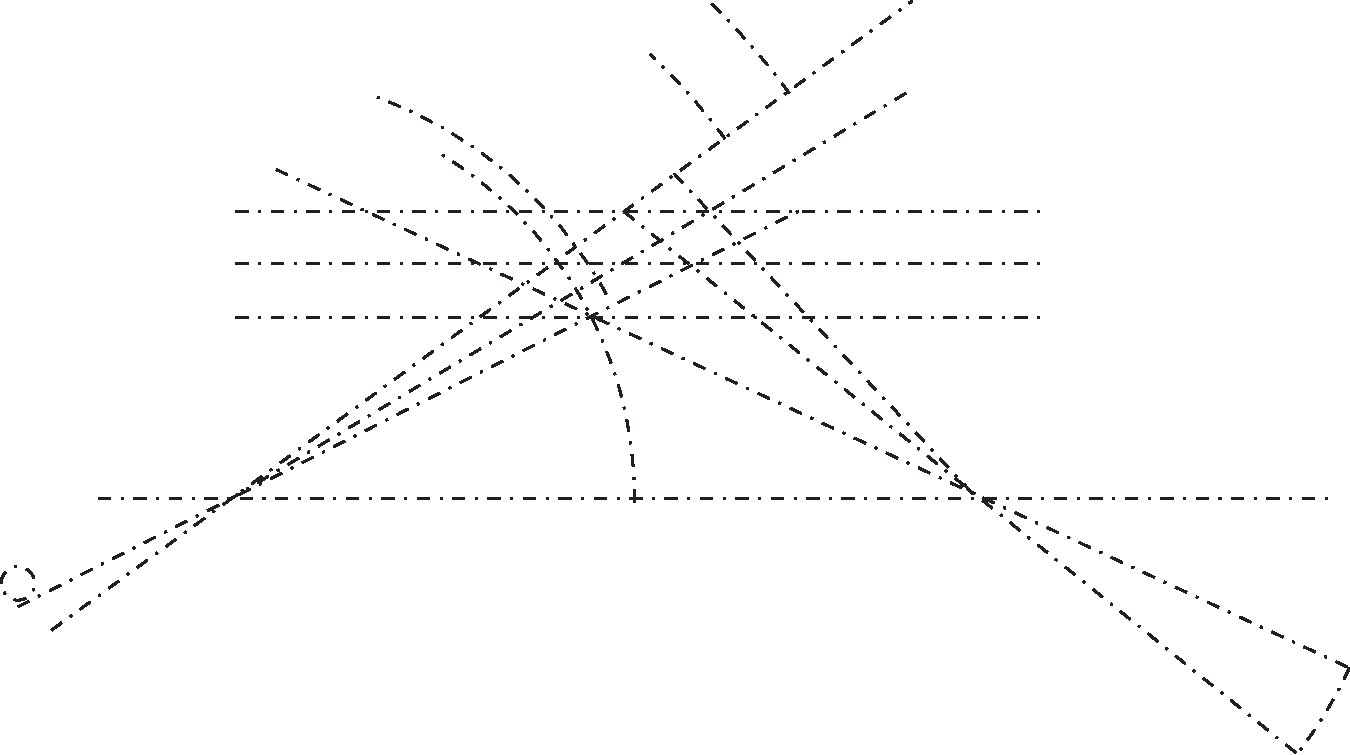
\includegraphics[width=0.6\textwidth]{images/LH037,03_078v-d1.pdf}\\
\centering[\textit{Fig. 1, Blindzeichnung}]
\pend
\newpage
\pstart
\centering 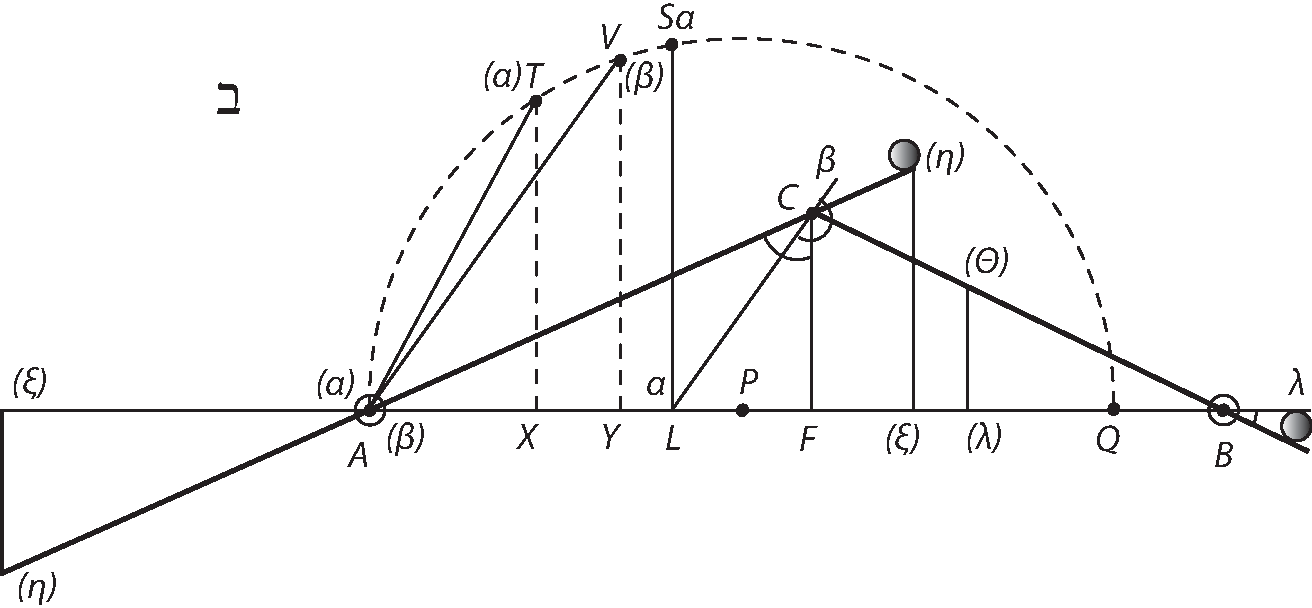
\includegraphics[width=0.9\textwidth]{images/LH037,03_078v-d2.pdf}\\
\centering [\textit{Fig. 2}]
\pend
\vspace{1.5em}
\pstart \noindent
\setline{1}(Eodem modo \rule[-4mm]{0mm}{10mm}$\displaystyle\frac{GH}{HC}=\frac{CF}{FN}=\frac{CF}{FL}.$)
Ergo $\displaystyle AR=AF+\frac{CF}{FL}$ et $DR=CF+1.$
\edtext{Quadratum $AR^{2}$}{\lemma{Quadratum}\Bfootnote{\textit{(1)}\ illius: \textit{(2)}\ $AR^{2}$ \textit{ L}}}
\rule[-4mm]{0mm}{10mm}$\displaystyle=AF^{2}+\frac{2FL}{CF}\cdot AF+\frac{FL^{2}}{CF^{2}}$ et $\medsquare$tum, $DR^{2}=$ 
\edtext{$CF^{2}+2CF+1.$ Erit}{\lemma{$CF^{2}+2CF+1.$}\Bfootnote{\textit{(1)}\ Denique $AG=AC=AF$ \textit{(2)}\ Erit \textit{ L}}} 
\rule[-4mm]{0mm}{10mm}$AD=\sqrt{\vphantom{\mathstrut \left\{AF^{2} + \displaystyle\frac{2FL}{CF} \cdot AF + \displaystyle\frac{FL^{2}}{CF^{2}} \atop CF^{2} + 2CF + 1 \right\}}} \displaystyle\left\{AF^{2} + \displaystyle\frac{2FL}{CF} \cdot AF + \displaystyle\frac{FL^{2}}{CF^{2}} \atop CF^{2} + 2CF + 1 \right\}$ \quad
%zwei Alternativen zu dieser Rechnung bzgl. des Wurzelstriches:
%$\displaystyle AD = \sqrt{\left\{AF^{2} + \frac{2FL}{CF} \cdot AF + \frac{FL^{2}}{CF^{2}} \atop CF^{2} + 2CF + 1 \right\}} \ AG =$
%$\displaystyle AD=\sqrt{\vphantom{\mathstrut \left\{AF^{2} + \frac{2FL}{CF} \cdot AF + \frac{FL^{2}}{CF^{2}} \atop CF^{2} + 2CF + 1 \right\}}} \left\{AF^{2} + \frac{2FL}{CF} \cdot AF + \frac{FL^{2}}{CF^{2}} \atop CF^{2} + 2CF + 1 \right\}$
\rule[-4mm]{0mm}{10mm}$AG=\sqrt{CF^{2} + AF^{2}}$ 
$\langle$\,\textendash\,\textendash\,\textendash\,$\rangle$
%$\displaystyle\frac{\left\{AF^{2} + \frac{2FL}{CF} \cdot AF + \frac{FL^{2}}{CF^{2}} \atop CF^{2} + 2CF + 1 \right\}}{\langle C\rangle F^{2}+AF^{2}}=\frac{DR}{GL}=\frac{1+CF}{GH+CF}.$
$\displaystyle\frac{\displaystyle\efrac{AF^{2} + \displaystyle\frac{2FL}{CF} \cdot AF + \displaystyle\frac{FL^{2}}{CF^{2}}}{CF^{2} + 2CF + 1}}{\langle C\rangle F^{2}+AF^{2}}=\frac{DR}{GL}=\frac{1+CF}{GH+CF}$
\edtext{quadretur, $\displaystyle \frac{1 + 2CF + CF^2}{GH^2 + 2GH\smallfrown CF + CF^2}$}{\lemma{}\Bfootnote{quadretur, \ \textbar \ fietque \textit{ gestr.}\ \textbar\ $\displaystyle \frac{1 + 2CF + CF^2}{GH^2 + 2GH\smallfrown CF + CF^2}$ \textit{L}}}
\rule[-4mm]{0mm}{10mm}multiplicetur per crucem,
%<calc-8>:
$\displaystyle\cancel{AF^2CF^2}\cancel{+ CF^4}+2FL, AF, CF+\cancel{2CF^3}+(FL)^2+\cancel{CF^2}+\parallel 2GH, CF\smallfrown AF^2,+2GH\smallfrown CF^3+(4GH\smallfrown FL \smallfrown AF)+(4GH, CF^2)+\rule[-4mm]{0mm}{10mm}(\frac{2GH\smallfrown FL^2}{CF})+(2GH\smallfrown CF)\parallel(GH^2 AF^2) +\rule[-4mm]{0mm}{10mm} (GH^2 CF^2)(\frac{2FL}{CF} AF, GH^2) + (2GH^2 CF) + (\frac{GH^2 FL^2}{CF^2}+(GH^2)=\langle\,\textendash\,\textendash\,\textendash\,\rangle\,\langle CF^2\cancel{+ 2CF^3}\\ \cancel{+C\rangle F^4}+(AF^2)+2AF^2CF+\cancel{AF^2CF^2}
\langle\,\textendash\,\textendash\,\textendash\,\rangle
%<calc-9>:
\langle2FL, AF, \cancel{\rangle CF} + 2GH \cancel{, CF}, AF^2 + 2GH, CF^{\cancel{3}2}$
\pend 
\newpage
\pstart 
Unde fit 
%<calc-10>:
\rule[-4mm]{0mm}{10mm}$\displaystyle\frac{\cancel{2}AF^2-\cancel{2}FL, AF}{AF^2 + CF^2} = GH = \frac{GH}{1} = \frac{GH}{DE}.$
%\vspace*{1mm}
$\langle$quadr$\rangle$atum $CA,$ ad rectangulum $AF\smallfrown AL.$
\rule[-4mm]{0mm}{10mm}$\displaystyle{\atop \begin{tikzpicture}\draw (0,0) rectangle (0.4,0.2);\end{tikzpicture}} \frac{CA^2}{AF ^\smallfrown AL} = \frac{DE}{GH} =$\rule[-4mm]{0mm}{10mm}
%\vspace*{1mm}
%\edtext{$\displaystyle\frac{A}{B}$\\ \indent Ex puncto $P$ medio ipsius $LF,$ radio $PA$ descri}{\lemma{$\frac{A}{B}$}\Bfootnote{ \textit{(1)}\ Sumatur $BP=LF$ et ex medio puncto ipsius $AP$ describ \textit{(2)}\ Ex [...] describatur \textit{ L}}}\edtext{batur circumferentia circuli cui occurrat}{\lemma{describatur}\Bfootnote{ \textit{(1)}\ circulus cujus \textit{(a)} occurra \textit{(b)} libram \textit{(2)}\ circumferentia [...] occurrat \textit{ L}}}
%circumferentia circuli, cui occurrat $LS$ perpendiculariter erecta ex $L.$ Ajo, ut aequilibrium sit potentias $AB$ fore in duplicata ratione $CA, SL$
%
\edtext{$\displaystyle\frac{A}{B}.$%
\newline%
\indent%
Ex puncto $P$ medio ipsius $LF,$ radio $PA$ describatur circumferentia circuli cui occurrat}{\lemma{$\displaystyle\frac{A}{B}.$}\Bfootnote{\textit{(1)}\ Sumatur $BP=LF$ et ex medio puncto ipsius $AP$ describ \textit{(2)}\ Ex puncto [...] describatur \textit{(a)}\ circulus cujus \textit{(aa)} occurra \textit{(bb)} libram \textit{(b)}\ circumferentia [...] occurrat\ \textit{L}}}
$LS$ perpendiculariter erecta ex $L.$ Ajo, ut aequilibrium\protect\index{Sachverzeichnis}{aequilibrium} sit potentias\protect\index{Sachverzeichnis}{potentia} $AB$ fore in duplicata ratione $CA, SL$
\edtext{vel translatis $AC,$ in $AV,$ et $SL$ in $XT,$ demissisque perpendicularibus $TX,$ et $VY,$ erunt $\displaystyle\frac{A}{B}=\frac{AY}{AX}.$}{\lemma{}\Bfootnote{vel translatis [...] $\displaystyle\frac{A}{B}=\frac{AY}{AX}$ \textit{ erg.} \textit{ L}}} 
\rule[-4mm]{0mm}{10mm}Cum enim sit $LP=PF$ erit $FQ=AL,$ et $LQ=AF$ ergo $\Square SL=
\begin{tikzpicture}
\draw (0,0) rectangle (0.4,0.2);
\end{tikzpicture}
\, ALQ=AF\smallfrown AL$ ergo 
%%%%%%%%%%%%%%%%%%%%%%%%%%%%%%%%%
%<calc-12>: 
\rule[-4mm]{0mm}{10mm}$\displaystyle\frac{A}{B} \left(= \frac{DE}{GH}\right)=$ 
\edtext{$\displaystyle\frac{CA^2}{SL^2}.$\\ \indent Ergo positis $A=B$, ut aequilibrium\protect\index{Sachverzeichnis}{aequilibrium} sit, opus est fieri $AC=SL$.}{\lemma{$\displaystyle\frac{CA^2}{SL^2}.$}\Bfootnote{ \textit{(1)}\ Videndum an posita $LF=FN,$ sit $\displaystyle\frac{SL}{LN}=\frac{CF}{FN}$ seu an $SL=2CF.$ Sed hoc falsum, indefinite \textit{(2)}\ Ergo \textit{(a)} eo demum casu \textit{(b)} positis \textit{(aa)} $AB$ \textit{(bb)} $A=B,$ \textit{(aaa)} et $AC=BC$ \textit{(bbb)} imo etiam alias semper \textit{(ccc)} ut aequilibrium\protect\index{Sachverzeichnis}{aequilibrium} sit, opus est fieri $AC=SL.$  \textit{(3)}\ Ergo [...] fieri $AC=SL.$ \textit{L}}}
\pend
\pstart
Idque problema\protect\index{Sachverzeichnis}{problema} per analysin solvi  
\edtext{potest ex data $AC$ et $X$ ratione}{\lemma{potest}\Bfootnote{ \textit{(1)}\ quaecunque ponatur ratio \textit{(2)}\ ex [...] ratione \textit{L}}}
ipsarum $AC, CB$ et posita
\edtext{$AC=CB.$ Similiter ex data ratione}{\lemma{$AC=CB.$}\Bfootnote{\textit{(1)}\ Et in genere ex datis  \textit{(2)}\ Similiter ex data ratione \textit{L}}} 
\edtext{seu}{\lemma{}\Bfootnote{seu \textit{erg.} \textit{L}}} 
\rule[-4mm]{0mm}{10mm}ponderum\protect\index{Sachverzeichnis}{pondus}
\edtext{$\displaystyle\frac{AC}{SL}$}{\lemma{}\Bfootnote{$\displaystyle\frac{AC}{SL}$ \textit{erg.} \textit{L}}} 
et ipsa $AF,$ vel ipsa $CF,$
\edtext{et $AC$}{\lemma{}\Bfootnote{et $AC$ \textit{erg.} \textit{L}}} 
\edtext{seu inveniri}{\lemma{}\Bfootnote{seu \ \textbar \ ex data ratione \textit{ gestr.}\ \textbar\ inveniri \textit{L}}}
poterit $CB$.
\pend
\pstart
\edtext{Esto $CA=\ $}{\lemma{}\Bfootnote{Esto $CA=$ \textit{erg.} \textit{L}}}$CB=a.\ CF=b$ erit $FB=
FB
\edtext{=AF}{\lemma{}\Bfootnote{$=AF$ \textit{erg.} \textit{L}}} 
=\sqrt{a^2 - b^2}$
qua si dividatur $b^2$ habebitur \rule[-4mm]{0mm}{10mm}$\displaystyle LF=\frac{b^2}{\sqrt{a^2 - b^2}}.$
Ejusque dimidium $\displaystyle PL
\edtext{=PF}{\lemma{}\Bfootnote{$=PF$ \textit{erg.} \textit{L}}} 
=\frac{b^2}{2 \sqrt{a^2 - b^2}}.$
Ergo $PA=PS
\edtext{=AF-PF}{\lemma{}\Bfootnote{$=AF-PF$ \textit{erg.} \textit{L}}}$ 
erit
\rule[-4mm]{0mm}{10mm}$\displaystyle\sqrt{a^2 - b^2} - \frac{b^2}{2 \sqrt{a^2 - b^2}} = \frac{2a^2 - 3b^2}{2 \sqrt{a^2-b^2}}$
et
$SL = \sqrt{PS^2 - PL^2}.$
Seu
\rule[-4mm]{0mm}{10mm}$\displaystyle\sqrt{\vphantom{\mathstrut \frac{4a^2 - 12a^2b^2 + 9b^4 - b^4}{4a^2 - 4b^2}}} \frac{4a^2 - 12a^2b^2 + 9b^4 - b^4}{4a^2 - 4b^2}=
\sqrt{\vphantom{\mathstrut \frac{a^4 - 3a^2b^2 + 2b^4}{a^2 - b^2}}} \frac{a^4 - 3a^2b^2 + 2b^4}{a^2 - b^2}
=CA=a.$
\pend
\begin{center}
%\vspace*{-3mm}
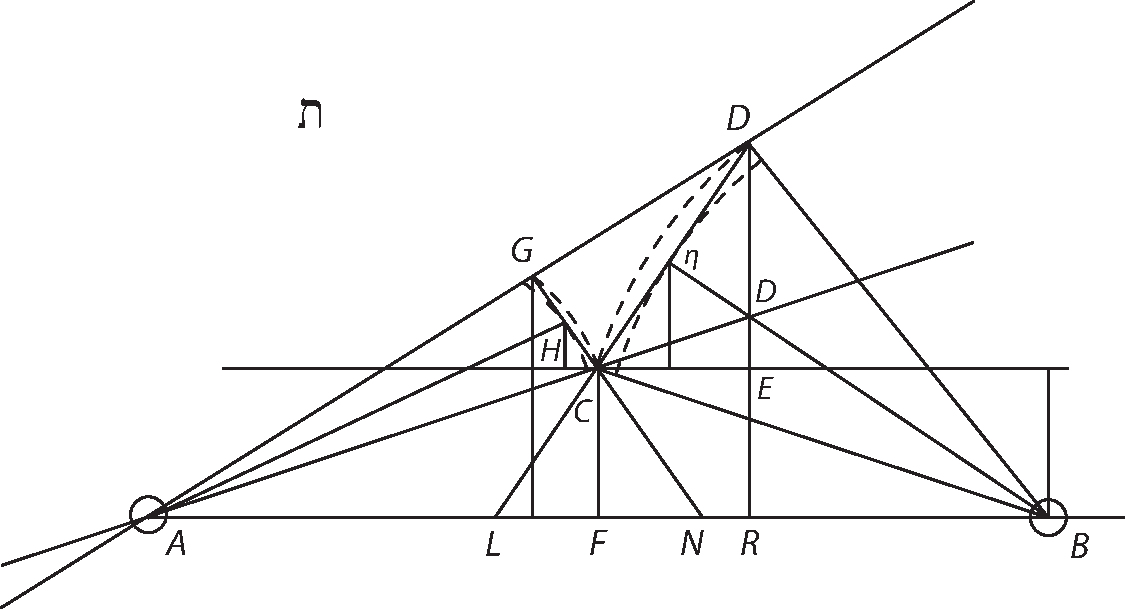
\includegraphics[width=0.85\textwidth]{images/LH037,03_078v-d3.pdf}\\
\lbrack\textit{Fig. 3}\rbrack
\end{center}
\vspace*{1.5em}
\pstart
Ecce ergo aequationem: 
\rule[-4mm]{0mm}{10mm}$\displaystyle\frac{a^4 - 3a^2b^2 + 2b^4}{a^2 - b^2} = a^2$.
\pend
\pstart\noindent
Ergo
$a^4 - 3a^2b^2 + 2b^4 = a^4 - b^2a^2.$ 
\pend
\pstart\noindent
\begin{wrapfigure}[7]{l}{0.22\textwidth}
%\hspace*{-4mm}
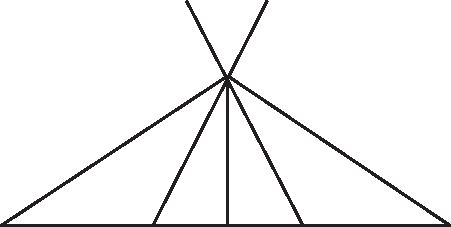
\includegraphics[trim = 0mm -5mm -3mm 0mm, clip, width=0.22\textwidth]{images/LH037,03_078v-d4.pdf}\\
\centering [\textit{Fig. 4}] 
\end{wrapfigure}
Ergo 
$-a^2b^2 + b^4 = 0,$
sive $a=b$ quod cum sit impossibile, nisi angulus \textit{ACB} sit minimus, sive rectae $AC, BC$ coincidant punctis $AB$ cadentibus in $F,$ et ipsis $AC, BC$ in unam rectam ex $F$ perpendiculariter erectam, ideo problema\protect\index{Sachverzeichnis}{problema} solvi non potest; ac nuspiam utcunque rationes aequilibrium\protect\index{Sachverzeichnis}{aequilibrium} erit $\langle$\,\textendash\,\textendash\,$\rangle$ $C,$ et $A=B,$ semperque 
$\langle$\,\textendash\,\textendash\,$\rangle$
$BC$ ascendet. 
$\langle$\,\textendash\,\textendash\,$\rangle$
cum continue de-
$\langle$\,\textendash\,\textendash\,$\rangle$
in elevatione
$\langle$\,\textendash\,\textendash\,$\rangle$
$\langle$cr$\rangle$escat. 
$\langle$\,\textendash\,\textendash\,$\rangle$
$\langle$m$\rangle$achina\protect\index{Sachverzeichnis}{machina}
$\langle$\,\textendash\,\textendash\,$\rangle$d
dum
$\langle$\,\textendash\,\textendash\,$\rangle$
accedant
$\langle$\,\textendash\,\textendash\,$\rangle$tur.
\pend
\pstart
$\langle$\,\textendash\,$\rangle$
$\langle$Si$\rangle$t eorum 
\edtext{$AC^2, SL^2$}{\lemma{}\Bfootnote{$AC^2, SL^2$ \textit{erg.} \textit{L}}} 
ratio 
$\langle$\,\textendash\,$\rangle$
\rule[-4mm]{0mm}{10mm}$\displaystyle\frac{\langle a^4 - 3a^2b^2\rangle + 2b^4}{\langle a^2 - b^2\rangle^2}=\gamma=\frac{B}{A}$
$\langle$\,\textendash\,$\rangle$ 
$\langle$p$\rangle$otes ut 
$\langle$\,\textendash\,$\rangle$
$\langle$com$\rangle$pendiosius
$\langle$\,\textendash\,$\rangle$ \lbrack78~r\textsuperscript{o}\rbrack\ 
\pend
\count\Afootins=1500
\count\Bfootins=1500
\count\Cfootins=1500
%\vspace*{-5mm}
%\begin{center}
%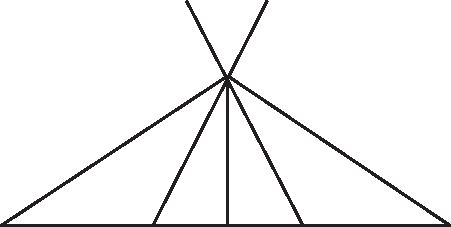
\includegraphics[width=0.4\textwidth]{images/LH037,03_078v-d4.pdf}\newline
%[\textit{Fig. 4}]
%\end{center}